%!TEX root = ../../csuthesis_main.tex

\chapter{基于通道注意力机制的CORnet-Z模型优化}

\section{CORnet模型复现与基线分析}

\subsection{复现流程与实验配置}

CORnet-S模型是类脑视觉建模中典型的时间递归结构模型,其引入“时间步”(time steps)以模拟视觉皮层多次循环加工过程。为验证该模型在轻量级图像分类任务中的性能表现,并为后续结构改进提供对照基线,本文在Tiny-ImageNet-200数据集上对CORnet-S进行了完整复现与训练。

Tiny-ImageNet-200是ImageNet数据集的轻量级衍生版本,包含200个类别,每个类别下含有500张训练图像、50张验证图像和50张测试图像,图像均为RGB三通道,分辨率为64×64,数据集总规模约为120000张\cite{le2015tiny}。相比较于原始ImageNet(包含1000个类别,超过120万张图像),Tiny-ImageNet在保留多类别识别任务结构的同时大幅减少了数据规模,显著降低了模型调试、验证和分析的训练成本,特别适合用于轻量级模型测试与类脑结构优化实验以及在硬件需求不足的情况下使用。

\begin{table}[htb]
	\centering
	\caption{Tiny-ImageNet 数据集结构与规模统计表}
	\label{tab:tinyimagenet}
	\begin{tabular}{lllll}
		\hline
		数据划分 & 类别数 & 每类图像数 & 总图像数 & 图像尺寸 \\
		\hline
		训练集(train) & 200 & 500  & 100,000  & 64 × 64 × 3 \\
		验证集(val)   & 200 & 50   & 10,000   & 64 × 64 × 3 \\
		测试集(test)  & 200 & —    & 10,000   & 64 × 64 × 3 \\
		\textbf{合计}   & \textbf{200} & — & \textbf{120,000} & — \\
		\hline
	\end{tabular}
\end{table}

从数据内容以及结构上来看,Tiny-ImageNet覆盖了自然场景中的动物、植物、器具、交通工具等多种类别,图像采集来源广泛,标注准确,是一个兼具语义多样性与任务完整性的视觉识别基准数据集。由于其类别标签与ImageNet synset保持一致,该数据集也可用于ImageNet预训练模型的微调与迁移学习实验,具有良好的通用性和拓展性。Tiny-ImageNet使用了严格的目录层级组织方式。训练集以每类一个子文件夹的形式存储图像,验证集与测试集通过单独的索引文件(val\_annotations.txt)提供图像路径与标签对应关系,方便使用PyTorch等深度学习框架进行批量加载与处理。

在数据预处理过程中,训练集图像首先进行了随机裁剪与随机水平翻转的增强操作,以提升模型对尺度与姿态变化的泛化能力。考虑到后续模型结构设计参考了ImageNet预训练风格,输入尺寸统一调整为$224×224$,标准化处理均值为$[0.485,0.456,0.406]$,标准差为$[0.229,0.224,0.225]$。

验证集和测试集则使用统一的中心裁剪策略,并统一缩放到$224×224$,以保证评估过程的稳定性,避免因数据增强带来的评估波动,确保模型在不同实验间具有可比性。所有图像在进入模型前均经过ToTensor( )转换并执行标准化处理,保持与ImageNet预训练模型输入风格一致。

在数据加载实现上,本文使用PyTorch框架中的ImageFolder接口对训练集与验证集目录进行加载,并分别设置了4个并行数据读取线程(num\_workers=4),有效缓解数据读取瓶颈对GPU训练过程的影响,提高训练效率。

本文使用原始CORnet项目中公开的CORnet-S模型结构代码,并基于Kubilius等人在NeurIPS 2019论文中发布的配置进行参数设定\cite{kubilius2019brain}。CORnet-S模型遵循生物视觉皮层的区域划分设计,主要包含四个模块(V1、V2、V4、IT),分别对应灵长类视觉通路的层级区域。其中,V2、V4和IT模块均内置时间步递归机制,输入图像会在多个时间步内重复处理,使模型具备“类再入处理”的表征能力。各时间步之间共享卷积核参数,从而避免模型参数量过多的膨胀问题,增强时间建模的稳定性。

模型的decoder部分由全局平均池化层与全连接线性层组成,用于对IT模块的输出特征图进行压缩与分类映射。考虑到模型初始结构是为ImageNet原始任务设计,输出维度被设定为1000,对应ImageNet的1000个语义标签。在本研究中,虽然实际使用的是Tiny-ImageNet数据集(共200类),但为保持与原项目训练流程的一致性,结构仍保留1000维输出,但后续仅使用其中200维参与分类损失计算。

损失函数采用PyTorch框架中标准的交叉熵损失(CrossEntropyLoss),用于多类别分类任务中的目标概率分布与预测输出之间的距离计算。该函数结合了softmax与negative log likelihood,有助于模型快速收敛于最优类别概率分布\cite{mao2023cross}。优化器选择动量随机梯度下降(SGD with momentum),初始学习率设置为0.1,动量系数为0.9,权重衰减系数为$1\times 10^{-4}$。动量项可以在训练过程中引入“惯性”,减少局部震荡,加快在鞍点附近的收敛速度,被广泛用于大型卷积神经网络的训练中\cite{sutskever2013importance}。为加快收敛并避免过拟合,采用步长为10的学习率衰减策略(StepLR),每训练10个epoch将学习率缩小10倍。这种阶梯式衰减策略对于避免后期训练陷入局部最优、提升模型稳定性具有实际效果。

本次训练过程共设置了43个epoch,batch size大小为256,与原始CORnet项目保持一致。训练使用单张NVIDIA RTX 3090 GPU,启用了cuDNN的自动优化模式(torch.backends.cudnn.benchmark = True),可根据输入张量尺寸动态选择最优的卷积算法,进一步提升训练加速效率\cite{paszke2019pytorch}。

为确保训练过程可追溯与结果可复现,每个epoch在验证集上进行一次准确率评估,记录Top-1与Top-5的准确率,并将训练日志、准确率曲线与模型状态以results.pkl文件格式存储。同时,模型权重在训练过程中定期保存至输出路径,方便后续中断恢复与版本比对分析。

\subsection{性能验证分析}

为验证复现后的CORnet-S模型在Tiny-ImageNet-200数据集上的分类能力,本文对训练过程中的模型性能进行了记录与分析。重点关注模型在验证集与训练集上的Top-1和Top-5准确率变化情况,以及损失函数的收敛趋势。

为更直观地展示模型在不同类别层级的识别能力,Top-1准确率用于衡量模型是否能准确预测图像的主类别标签,而Top-5准确率则反映模型是否将正确类别包含在前5个高置信度预测中。在Tiny-ImageNet这类小样本多类别任务中,Top-5准确率常作为模型泛化能力的重要参考指标。

\begin{figure}[hbt]
	\centering
	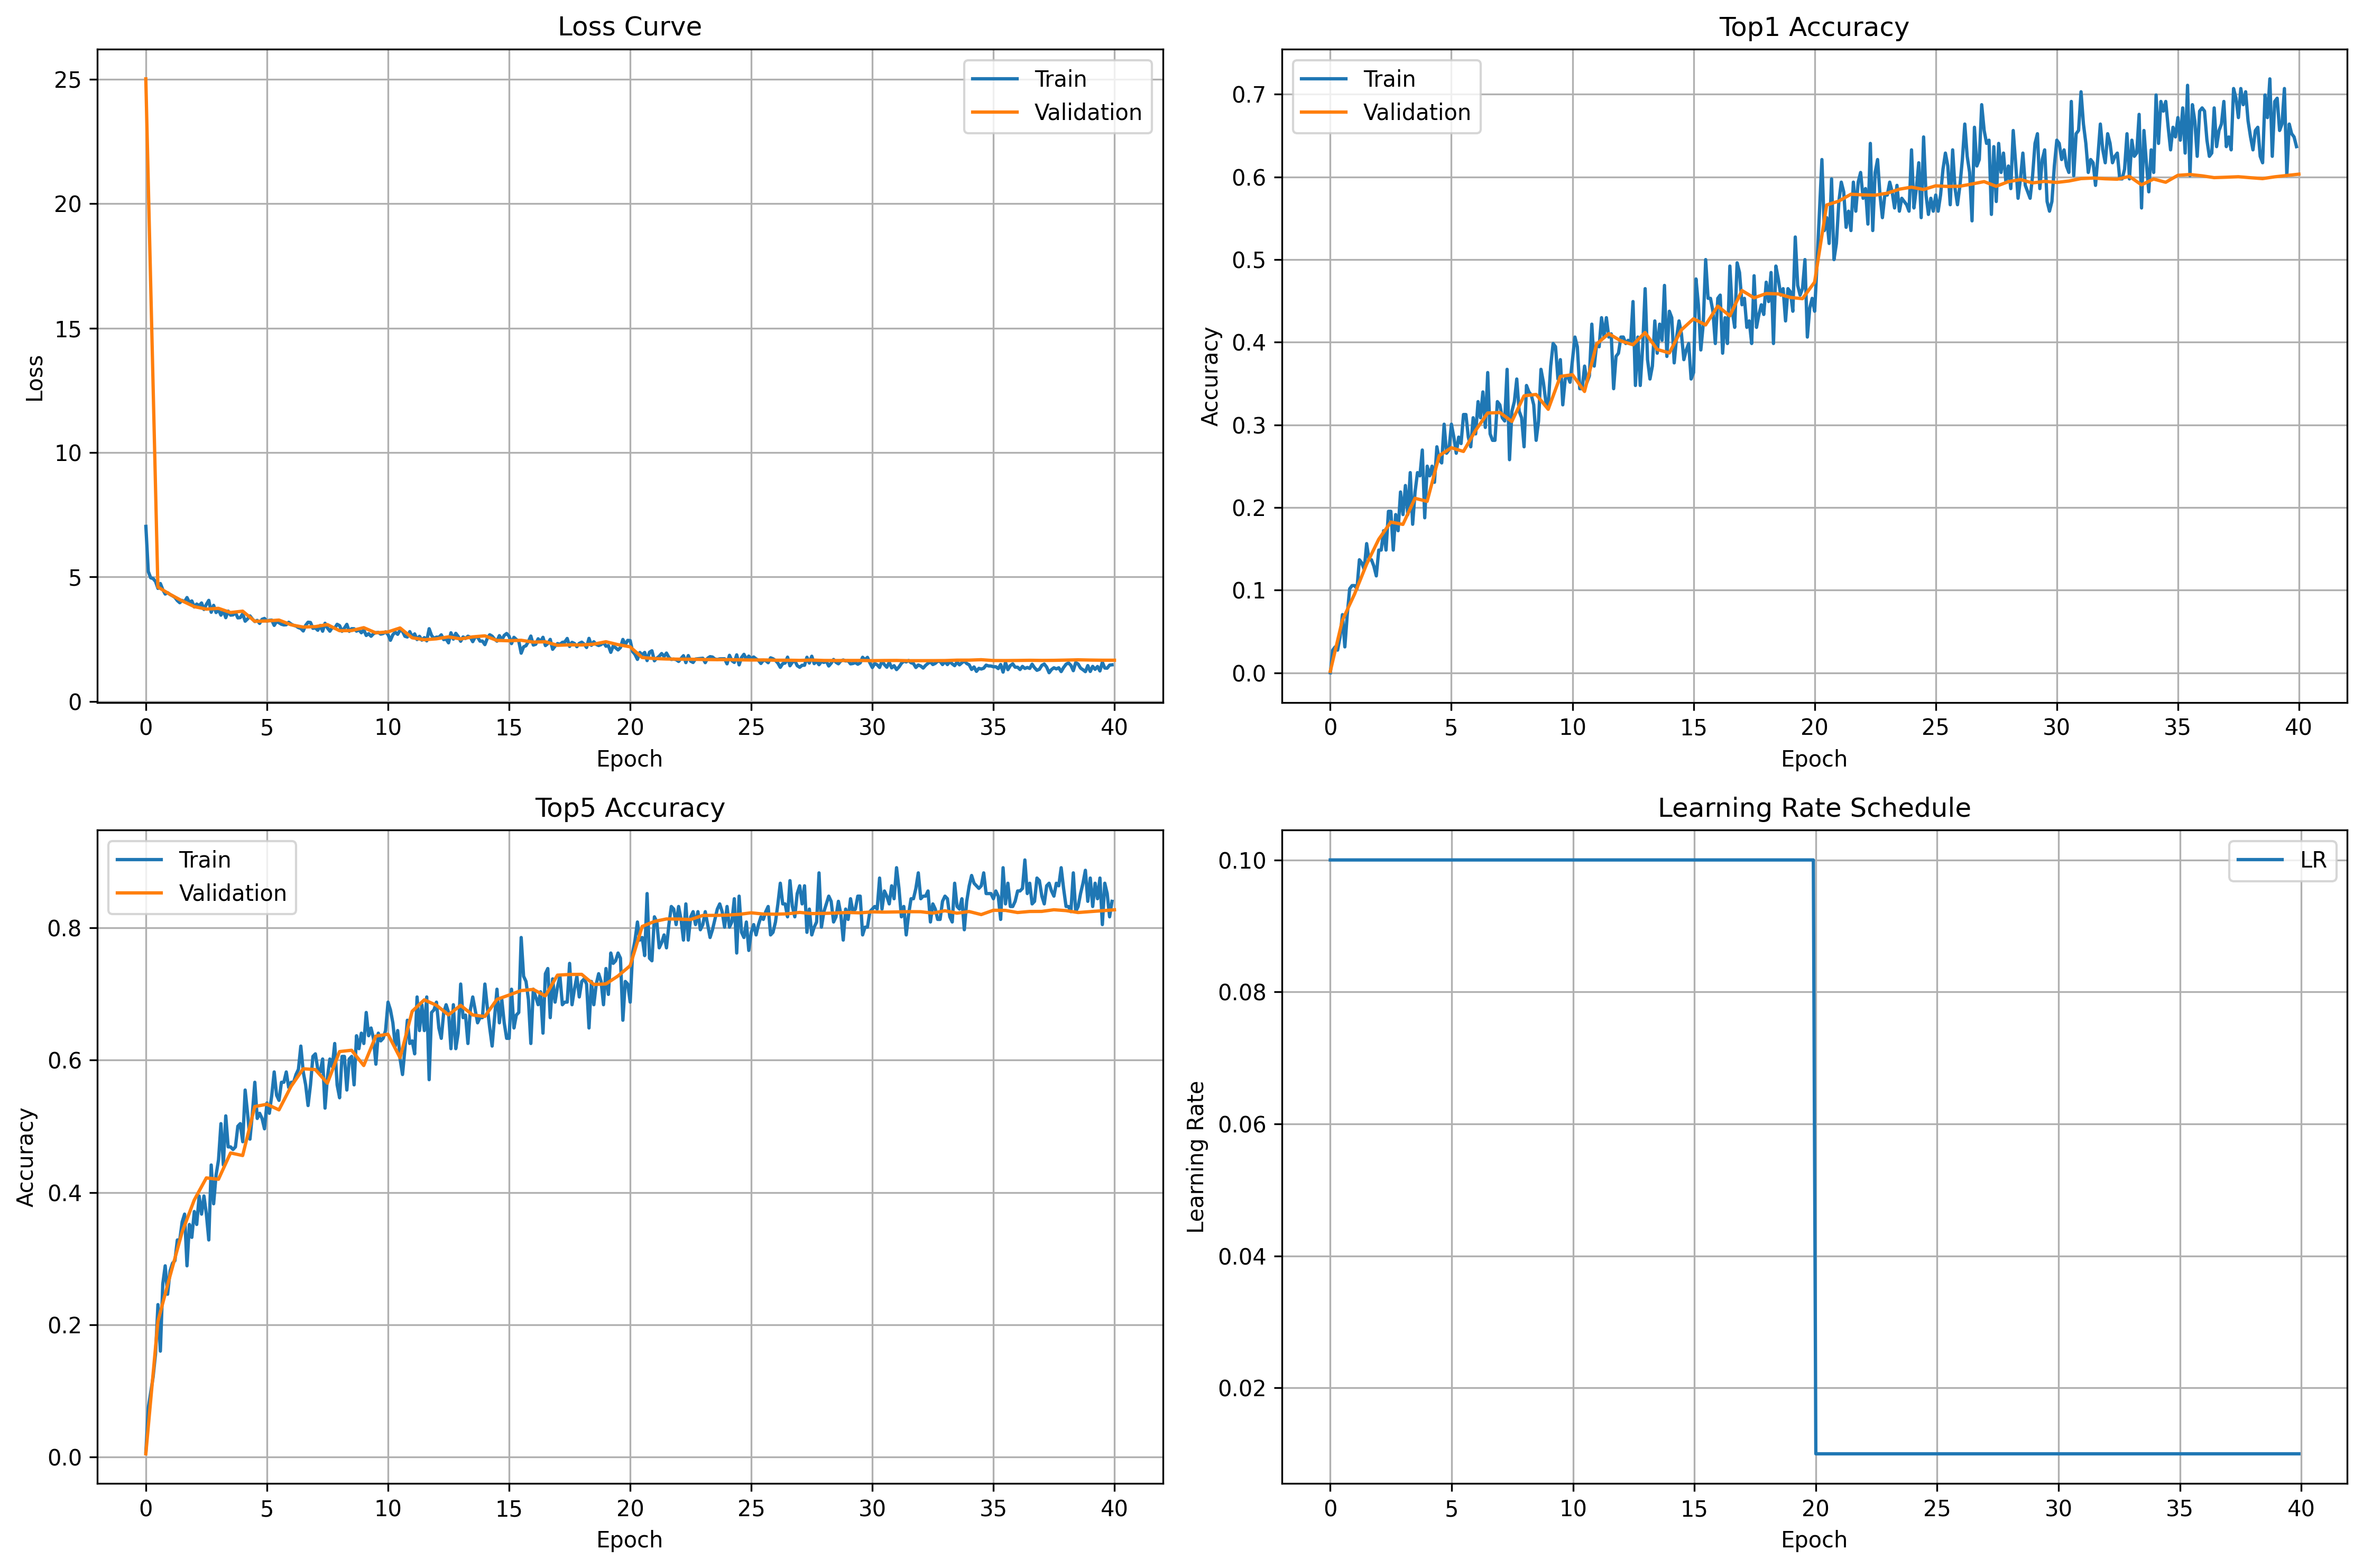
\includegraphics[width=0.9\linewidth]{cornet-s.png}
	\caption{CORnet-S训练数据变化图}
	\label{f.szxt}
\end{figure}

如图\ref{f.szxt}所示,在训练40个epoch后,模型达到其在验证集上的最佳表现。验证结果显示,模型的Top-1准确率为60.34\%,Top-5准确率为82.70\%,对应的交叉熵损失为1.6567。与此同时,模型在训练集上的Top-1准确率为63.67\%,Top-5准确率为83.98\%,训练损失为1.4718。验证集与训练集的准确率差距较小,表明模型在当前配置下未出现明显的过拟合现象,训练过程较为稳定。

原始的CORnet-S模型由Kubilius等人于2019年在NeurIPS会议中提出,其在ImageNet数据集上的Top-1准确率为74.4\%\cite{kubilius2019brain},在维持较小参数量的前提下,表现出接近ResNet-50的分类性能。同时,该模型在Brain-Score框架下的IT区神经预测得分也很高,被视为在准确率与类脑性之间达到较好平衡的代表性架构。

本文在Tiny-ImageNet-200数据集上复现了该类脑视觉模型,并使用标准训练配置进行训练与评估,最终在验证集上获得60.34\%的Top-1准确率和82.70\%的Top-5准确率。尽管该结果无法直接与原论文的ImageNet实验对齐,但在样本数量较少、图像尺寸较低的前提下,模型依然展现出稳定的识别能力,说明其结构在小样本多类别任务中同样具有较强适应性。

\begin{table}[htb]
	\centering
	\caption{CORnet-S准确率对比表}
	\label{tab:CORnet-S}
	\begin{tabular}{lllll}
		\hline
		       & 原始CORnet-S & 本文复现的CORnet-S \\
		\hline
		TOP1准确率 & 74.4\% & 60.34\%   \\
		TOP5准确率 & — & 82.70\%    \\
		\hline
	\end{tabular}
\end{table}

需要指出的是,Tiny-ImageNet的难度相较于完整的ImageNet仍有显著差异,类别缩减和图像简化可能会使模型更容易收敛。因此本实验的结果更多用于结构复现与改进对照,不可与完整ImageNet上的结果直接类比。但整体表现仍验证了CORnet-S模型在轻量级视觉任务中的有效性,也为后续结构优化与注意力机制集成提供了可靠的基线。

\subsection{基线可视化分析}

为分析模型在各视觉皮层模拟层级的特征提取情况,本文使用forward hook方法提取了CORnet-S模型各层的中间激活图,并对典型通道的响应特征进行了可视化。

\begin{figure}[hbt]
	\centering
	
\includegraphics[width=0.6\linewidth]{car.jpg}
	\caption{激活图原图像}
	\label{f.car}
\end{figure}


在本实验中,选择CORnet-S模型的IT层作为可视化目标层,对验证集中典型图像样本进行激活响应分析。图\ref{f.cornet_s_jihuo}的(d)展示了该模型在IT层的六个典型通道的激活结果。

\begin{figure}[!htb]
	\centering
	\begin{subfigure}[t]{0.8\linewidth}
		\captionsetup{justification=centering}
		\begin{minipage}[b]{1\linewidth}
			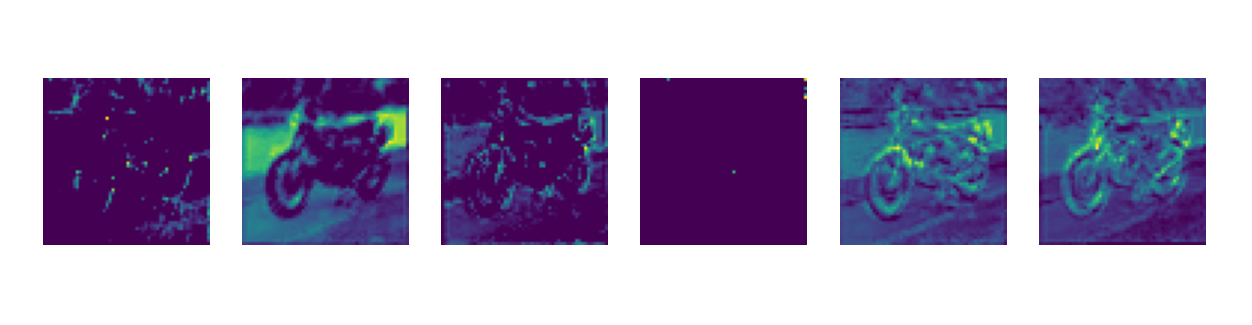
\includegraphics[width=1\linewidth]{V1_s_activations.png}
			\caption{V1层激活图}
		\end{minipage}
	\end{subfigure}\\
	\begin{subfigure}[t]{0.8\linewidth}
		\captionsetup{justification=centering}
		\begin{minipage}[b]{1\linewidth}
			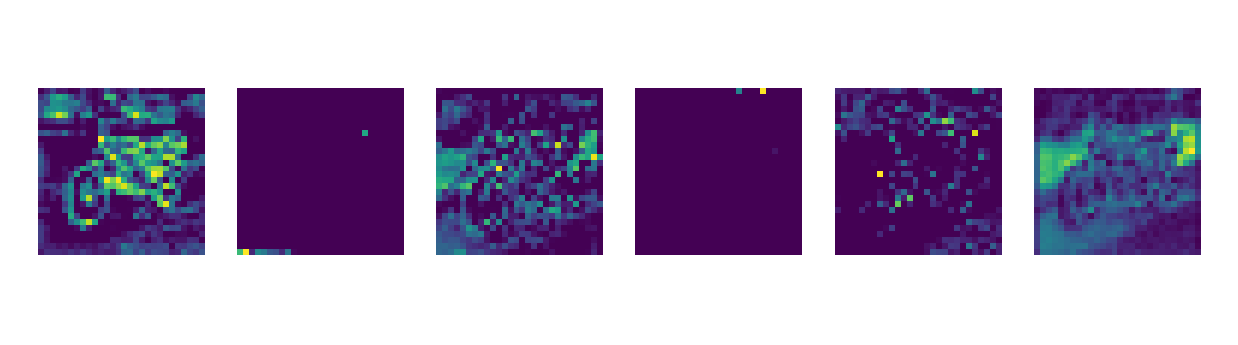
\includegraphics[width=1\linewidth]{V2_s_activations.png}
			\caption{V2层激活图}
		\end{minipage}
	\end{subfigure}\\
	\begin{subfigure}[t]{0.8\linewidth}
		\captionsetup{justification=centering}
		\begin{minipage}[b]{1\linewidth}
			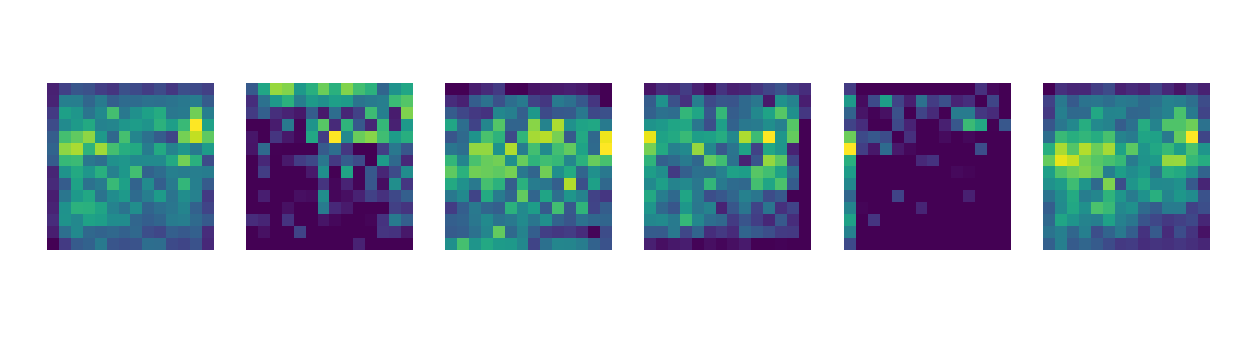
\includegraphics[width=1\linewidth]{V4_s_activations.png}
			\caption{V4层激活图}
		\end{minipage}
	\end{subfigure}\\
	\begin{subfigure}[t]{0.8\linewidth}
		\captionsetup{justification=centering}
		\begin{minipage}[b]{1\linewidth}
			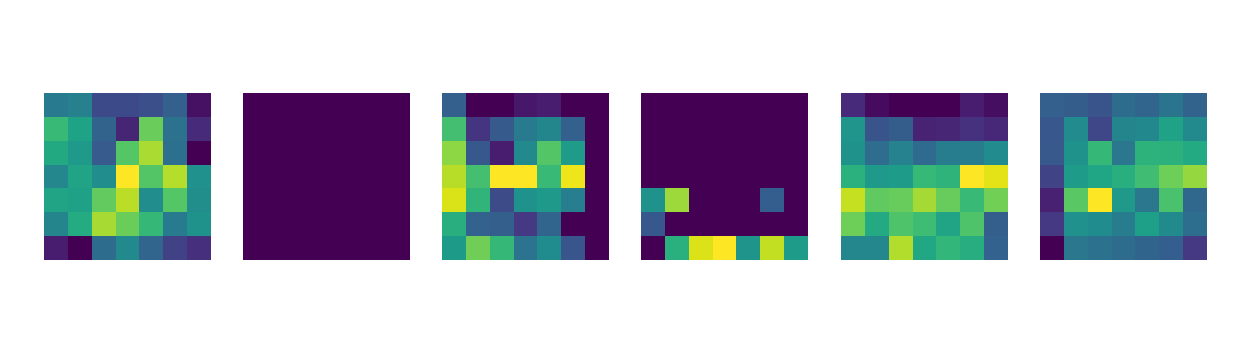
\includegraphics[width=1\linewidth]{IT_s_activations.png}
			\caption{IT层激活图}
		\end{minipage}
	\end{subfigure}
	\caption{CORnet-S模型各层激活图}
	\label{f.cornet_s_jihuo}
\end{figure}

观察图像可见,模型在多个通道中对图像主体区域(如摩托车轮廓、前轮等)产生了高响应,说明IT层能够聚焦于具有显著判别力的高阶语义特征。此外,部分通道对图像边缘或背景响应较弱,进一步印证该层在完成判别任务时具备一定的空间注意能力。

为进一步分析CORnet-S模型在不同层级的感知能力,图\ref{f.cornet_s_jihuo}的(a)至图\ref{f.cornet_s_jihuo}的(c)分别展示了模型在V1、V2和V4层的激活热力图。

从图\ref{f.cornet_s_jihuo}的(a)V1层可见,激活图主要集中在边缘与纹理区域,这表现出V1层为对图像整体结构的低级响应,体现了模型底层的感知特性。图\ref{f.cornet_s_jihuo}的(b)V2层中,响应区域虽仍零散,但开始聚焦于目标内部轮廓区域,初步展现出类别相关的空间感知。图\ref{f.cornet_s_jihuo}的(c)V4层显示出更集中的激活分布,尤其在图像的中部主体区域有明显增强,说明模型已完成对部分中层语义信息的整合。

尽管整体趋势符合生物视觉系统的层级响应特征,但部分激活图仍存在注意力漂移现象,如V1层的通道2与V2层的通道六对背景产生了强响应。这可能反映出当前模型在缺乏显式注意机制的条件下,其选择性聚焦能力存在一定的偏移,尤其在目标边界模糊、遮挡或图像背景复杂的场景下。

综上所述,激活图可视化结果表明,CORnet-S模型具有基本的空间关注能力和层级特征提取结构,但在判别区域的集中性与鲁棒性方面仍有改进空间。后续章节将尝试引入通道注意力机制,进一步优化模型对关键区域的响应特性。

\section{注意力机制的引入动因}

在前述CORnet-S和CORnet-Z的模型结构中,各模块的特征提取过程采用标准卷积网络设计,未显式引入注意力调节机制。虽然该类模型在识别准确率与类脑性评估方面已具备一定表现,但在应对复杂图像背景、多目标干扰及特征稀疏性等问题时,模型关注能力有限,仍然存在注意力分配不足、无关区域激活过强的问题,导致信息利用效率降低,模型鲁棒性不足。

从神经科学的角度看,生物视觉系统能够通过注意力机制对有限的神经资源进行动态分配,这是感知过程中至关重要的一环。已有大量神经生理研究表明,大脑皮层不同层级的神经区域在视觉处理中表现出显著的选择性响应特征。例如,初级视觉皮层V1中的神经元更倾向于响应边缘、方向等低阶特征;而中层V4与高级区域IT则更侧重于颜色、形状和语义信息的整合处理。当个体的注意力被主动或被动地引导至某一目标区域时,与该区域相关的神经通道的活动将被显著增强,而与任务无关的信息通道则呈现出明显的抑制效应,这一机制称为“选择性增强/抑制”(selective enhancement/suppression)\cite{dicarlo2012does}。

为了模拟这一生物学机制,计算机视觉领域逐步发展出了多种注意力机制模块。Squeeze-and-Excitation(SE)模块的设计正是受这一神经调控模式启发。该模块通过“压缩”(squeeze)操作对空间维度进行全局信息整合,并通过“激励”(excitation)机制计算各通道的重要性分布,从而动态调整特征通道的响应强度,增强与目标任务相关的通道响应,抑制冗余干扰,具有高度类脑性的通道选择性功能\cite{hu2018squeeze}。

为此,本文在CORnet-Z模型基础上通过引入通道注意力机制(SE)模块,旨在提升模型对关键特征的感知能力和抗干扰能力,以更好地模拟神经系统的通道调控行为。这种结构调整有望在不显著增加模型复杂度的情况下,增强其在类脑评估任务中的表现一致性和识别准确率。

从工程实践的角度看,传统的卷积神经网络模型在图像特征提取过程中普遍存在通道响应冗余与表征不具判别性的问题,尤其在网络结构相对浅层或轻量化模型中更为突出。这种问题主要表现为:网络在不同通道上学习到的特征可能存在较强相关性或信息重复,缺乏对关键类别特征的显著响应,从而导致计算资源浪费和模型性能瓶颈\cite{he2016deep}。具体而言,当模型对所有通道“一视同仁”地处理输入信息时,会在训练过程中平均分配注意力,导致有用特征通道未能获得足够强化,反而部分背景噪声或低语义信息通道被不必要地激活。这种响应冗余不仅增加了模型计算负担,还在推理阶段引入了错误响应风险,降低了分类准确率与泛化能力,特别在面对遮挡、复杂背景与小样本类别时表现尤为明显\cite{wang2020eca}。

针对上述问题,近年来研究者提出了多种注意力机制,以提升特征通道的筛选能力。通道注意力机制通过自动学习各通道的重要性分布,实现特征向量的“压缩与选择”,有效抑制无效激活、增强关键特征表达。其中,SE模块作为一种结构紧凑、参数极少的轻量级注意力机制,凭借其不引入额外空间维度、易于与主干网络并联嵌套的优势,在ResNet、MobileNet等主流网络中广泛应用\cite{hu2018squeeze}。SE模块通过两个阶段完成注意力权重的生成:首先在“Squeeze”阶段对每个通道进行全局平均池化,提取全局上下文信息;随后在“Excitation”阶段通过两层全连接网络学习非线性通道权重,并以Sigmoid函数输出注意力分布。最终,模型将原始特征图按通道注意力进行重新加权,实现“信息压缩+特征增强”的组合表达机制。这一设计思想与生物视觉系统中“有限资源优先调动”机制具有一定类脑对照性。

在多类目标混合、背景复杂的Tiny-ImageNet数据集上,模型对高层语义特征的表征能力直接决定了其分类效果。该数据集每类图像数量较少、类别间相似度高,模型必须有效区分小尺度目标与大背景之间的细粒度差异,传统卷积提取器在此场景中往往难以充分表达判别信息。本文在CORnet-Z模型的V4或IT层引入SE模块,目的就是在保持结构轻量性的同时,增强模型对关键语义区域的响应能力,提高特征稀疏性与判别强度。

实验结果表明,引入SE模块后模型在Top-1与Top-5准确率上均有所提升,说明通道选择性机制能够在高层抽象阶段有效强化目标核心区域特征表达,为后续类脑性一致性分析提供了优化基础。

\section{通道注意力模块设计与集成}

\subsection{SE结构原理与实现}

为了增强CORnet-Z模型在图像识别过程中的通道选择能力,本文在原始模型结构的基础上引入通道注意力SE模块,构建了改进模型CORnet-Z+SE。该机制通过显式建模通道之间的依赖关系,实现对冗余特征的压制与有效特征的增强,从而提升模型的判别能力与可解释性。

SE模块由Hu等人于2018年提出\cite{hu2018squeeze},其核心思想就是通过两个阶段实现特征通道的重要性建模:squeeze(压缩)与 excitation(激励)。

在 squeeze 阶段,模块对输入特征图的每个通道进行全局平均池化,得到一个通道描述向量,压缩掉空间维度:

\begin{equation}
	z_c = 
	\frac{1}{H \times W} 
	\sum_{i=1}^{H} \sum_{j=1}^{W} x_c(i, j)
	\label{eq:se_squeeze}
\end{equation}
其中,$x_c(i,j)$表示输入特征图第$c$个通道在位置$(i,j)$的值,$z_c$为池化后通道$c$的全局描述,$H$和$W$分别为特征图的空间尺寸大小。

在excitation阶段,该通道向量$z$经过一个由两个全连接层组成的非线性变换,输出通道注意力权重向量$s$:

\begin{equation}
	s = \sigma \left( W_2 \cdot \text{ReLU} \left( W_1 \cdot z \right) \right)
	\label{eq:se_excitation}
\end{equation}
其中,$W_1 \in \mathbb{R}^{\frac{C}{r} \times C}$和$W_2 \in \mathbb{R}^{C \times \frac{C}{r}}$是两层全连接层的权重矩阵,$r$为压缩比超参数,用于控制中间层维度大小;$\text{ReLU}(\cdot)$表示线性整流函数,$\sigma(\cdot)$ 为Sigmoid 激活函数,用于将权重归一化到$[0,1]$区间。

最后,将注意力权重向量$s$与原始特征图逐通道相乘,完成对输入特征的加权重标定:

\begin{equation}
	\tilde{x}_c = s_c \cdot x_c
	\label{eq:se_scale}
\end{equation}
其中,$\tilde{x}_c$表示重标定后的通道特征图,$s_c$为通道$c$的注意力系数。通过这一机制,SE模块能够提升模型对目标区域特征的响应能力,增强判别特性。

在本文的实现中,使用PyTorch编写的\texttt{SEBlock}类对上述结构进行了复现。池化操作采用\texttt{nn.AdaptiveAvgPool2d(1)},全连接层使用两层\texttt{Linear}模块分别对应压缩与激励过程,激活函数为ReLU和Sigmoid。参数初始化方面,前层使用\texttt{kaiming\_normal\_},后层采用\texttt{normal\_}方法,以保证训练初期的稳定性。不同于原始论文中默认的压缩比$r=16$,本文选用更小的压缩比$r=8$,以减小信息损失并提高特征保持能力,使模块更适配于CORnet-Z这种浅层轻量模型结构。

\subsection{模块集成方式及参数配置}

在原始的CORnet-Z模型中,V1、V2、V4、IT四个模块以前馈方式逐层堆叠,每层结构为:Conv→ReLU→MaxPool。为在不重构网络的前提下集成注意力机制,本文在每一层中插入了SE模块,嵌入位置为:Conv→ReLU→SE→MaxPool。

即先进行特征提取与非线性激活,再由SE模块完成通道加权,最后下采样。此结构在\texttt{CORblock\_Z}中统一实现,并通过在初始化时设置\texttt{use\_se=True}启用。

各模块的通道设置如下表所示:

\begin{table}[htb]
	\centering
	\caption{CORnet-Z+SE各模块通道表}
	\label{tab:CORnet-Z+SE各模块通道表}
	\begin{tabular}{lllll}
		\hline
		模块& 输入通道 & 输出通道 \\
		\hline
		V1 & 3 & 64   \\
		V2 & 64 & 128   \\
		V4 & 128 & 256   \\
		IT & 256 & 512    \\
		\hline
	\end{tabular}
\end{table}

SE模块的参数均可被端到端训练自动学习,无需引入额外损失函数。集成后的模型结构保持可解释性良好,推理开销略高于原始的CORnet-Z模型,适用于中小型数据集(如Tiny-ImageNet-200)下的轻量化分类任务。

在模型训练中,保持原始CORnet-Z模型的训练策略不变,仅在结构上增加注意力机制,便于与原始模型在准确率与类脑性得分上进行对比分析。

\section{改进模型训练与性能表现}

\subsection{准确率与损失表现分析}

为评估所引入通道注意力机制对模型性能的实际影响,本文将改进后的CORnet-Z+SE模型与原始的CORnet-Z模型在Tiny-ImageNet-200数据集上的训练结果进行了系统对比与分析。重点分析模型在分类准确率、损失值以及收敛速度等方面的变化,用以验证SE模块的有效性。

在相同训练轮数范围内,原始的CORnet-Z模型在验证集上的Top-1准确率为32.51\%,Top-5准确率为59.21\%,对应的验证损失为2.9498。训练集表现略低,Top-1准确率仅为30.08\%,说明模型学习能力有限,可能存在梯度传播不充分或高层特征不具判别性的问题。

引入SE模块后的CORnet-Z+SE模型,在验证集上的Top-1准确率提升至36.66\%,Top-5准确率为62.72\%,损失下降至2.7265;训练集表现提升更为明显,Top-1准确率为35.94\%,Top-5准确率达64.84\%。验证与训练损失同步下降,说明注意力机制有效增强了模型的收敛能力和判别表达力。

\begin{table}[htb]
	\centering
	\caption{CORnet-Z与CORnet-Z+SE模型最佳性能表现对比}
	\label{tab:CORnet-Z与CORnet-Z+SE模型最佳性能表现对比}
	\begin{tabular}{lllll}
		\hline
		指标& CORnet-Z & CORnet-Z+SE \\
		\hline
		验证集Top-1准确率 & 32.51\% & 36.66\%  \\
		验证集Top-5准确率 & 59.21\% & 62.72\%  \\
		验证集损失值 & 2.9498 & 2.7265  \\
		训练集Top-1准确率 & 30.08\% & 35.94\%  \\
		训练集Top-5准确率 & 52.34\% & 64.84\%  \\
		训练集损失值 & 3.2815 & 2.7199  \\
		\hline
	\end{tabular}
\end{table}

从图像可视化分析来看,原始CORnet-Z模型如图\ref{f.zzxt}在训练过程中出现了较大的波动,尤其是Top-1准确率曲线抖动明显,表明模型的收敛过程不够平稳。而CORnet-Z+SE模型图\ref{f.zsezxt}在Top-1和Top-5准确率的上升曲线中的表现相较来说波动幅度更小,训练过程更稳定,验证集与训练集的性能差距也明显缩小,说明注意力机制的引入有助于特征通道的收敛与泛化。

同时,损失函数曲线(Loss Curve)也显示出一致趋势:原始的CORnet-Z模型在训练早期下降速度更快,但是最终损失值却略高,而且CORnet-Z原始模型在第5\textasciitilde10个epoch后出现训练集损失震荡,可能反映出部分通道未能有效建模关键区域。

\begin{figure}[hbt]
	\centering
	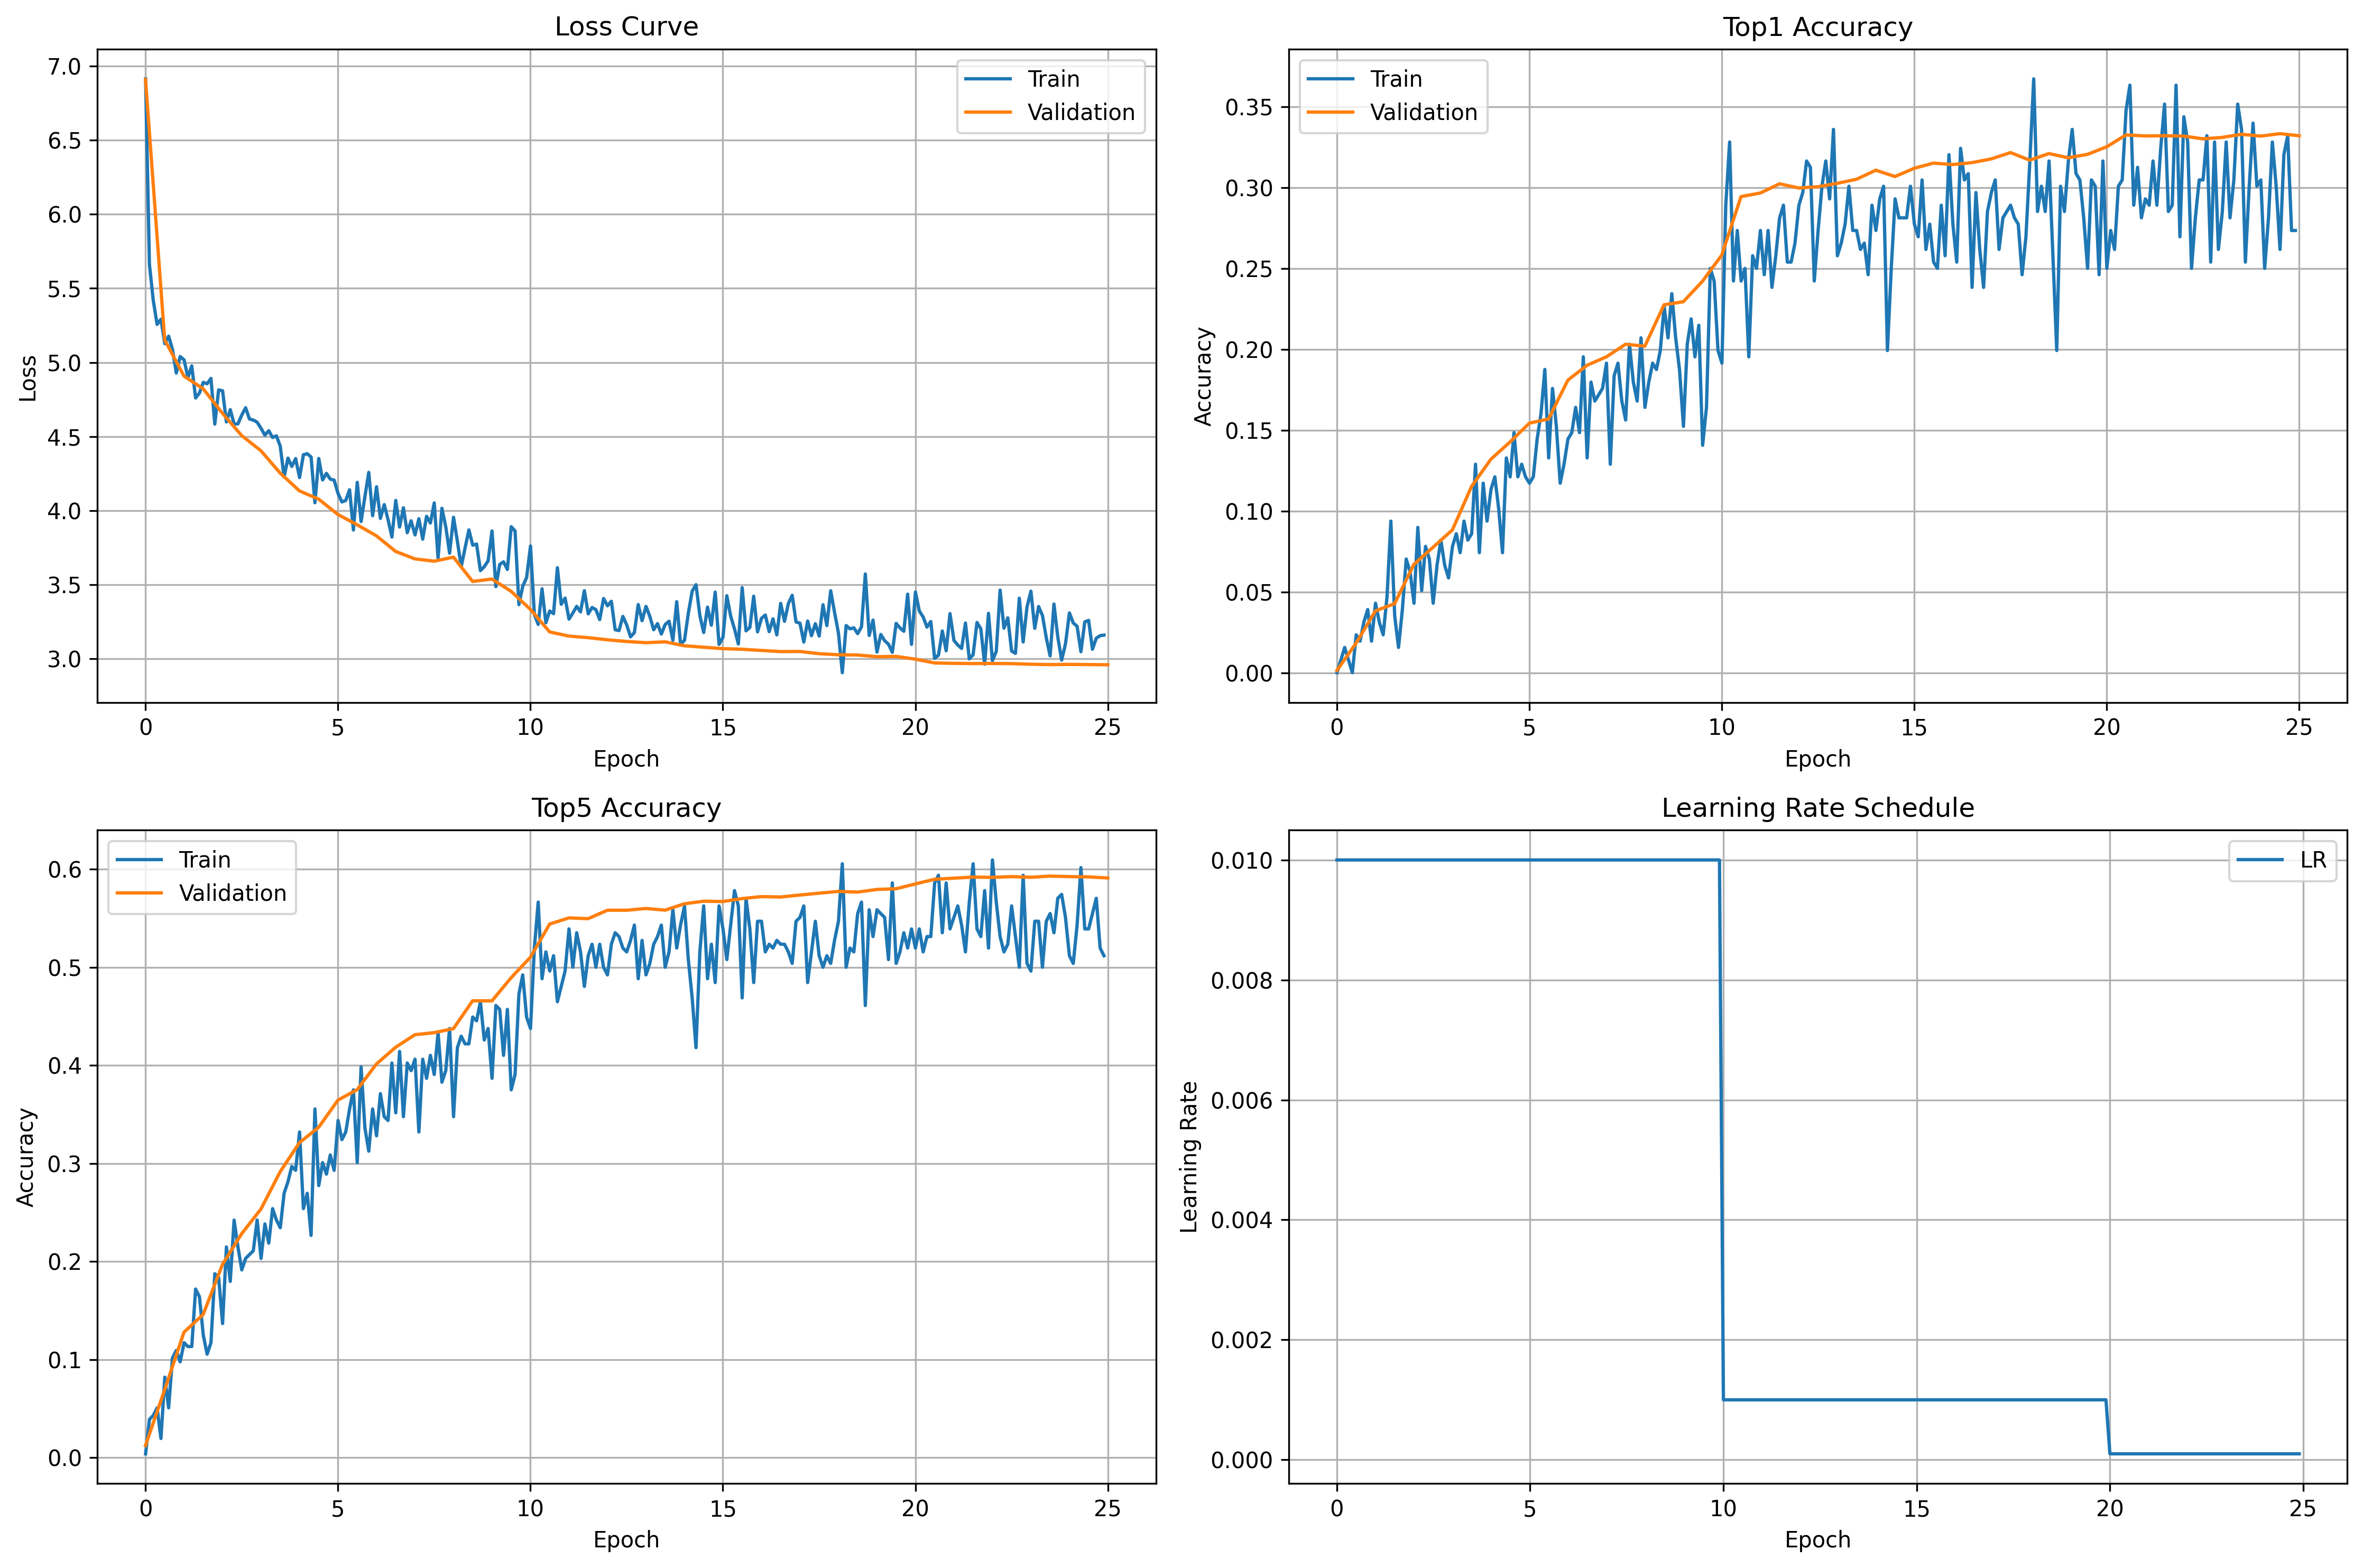
\includegraphics[width=0.9\linewidth]{cornet-z.png}
	\caption{CORnet-Z训练数据变化图}
	\label{f.zzxt}
\end{figure}

\begin{figure}[hbt]
	\centering
	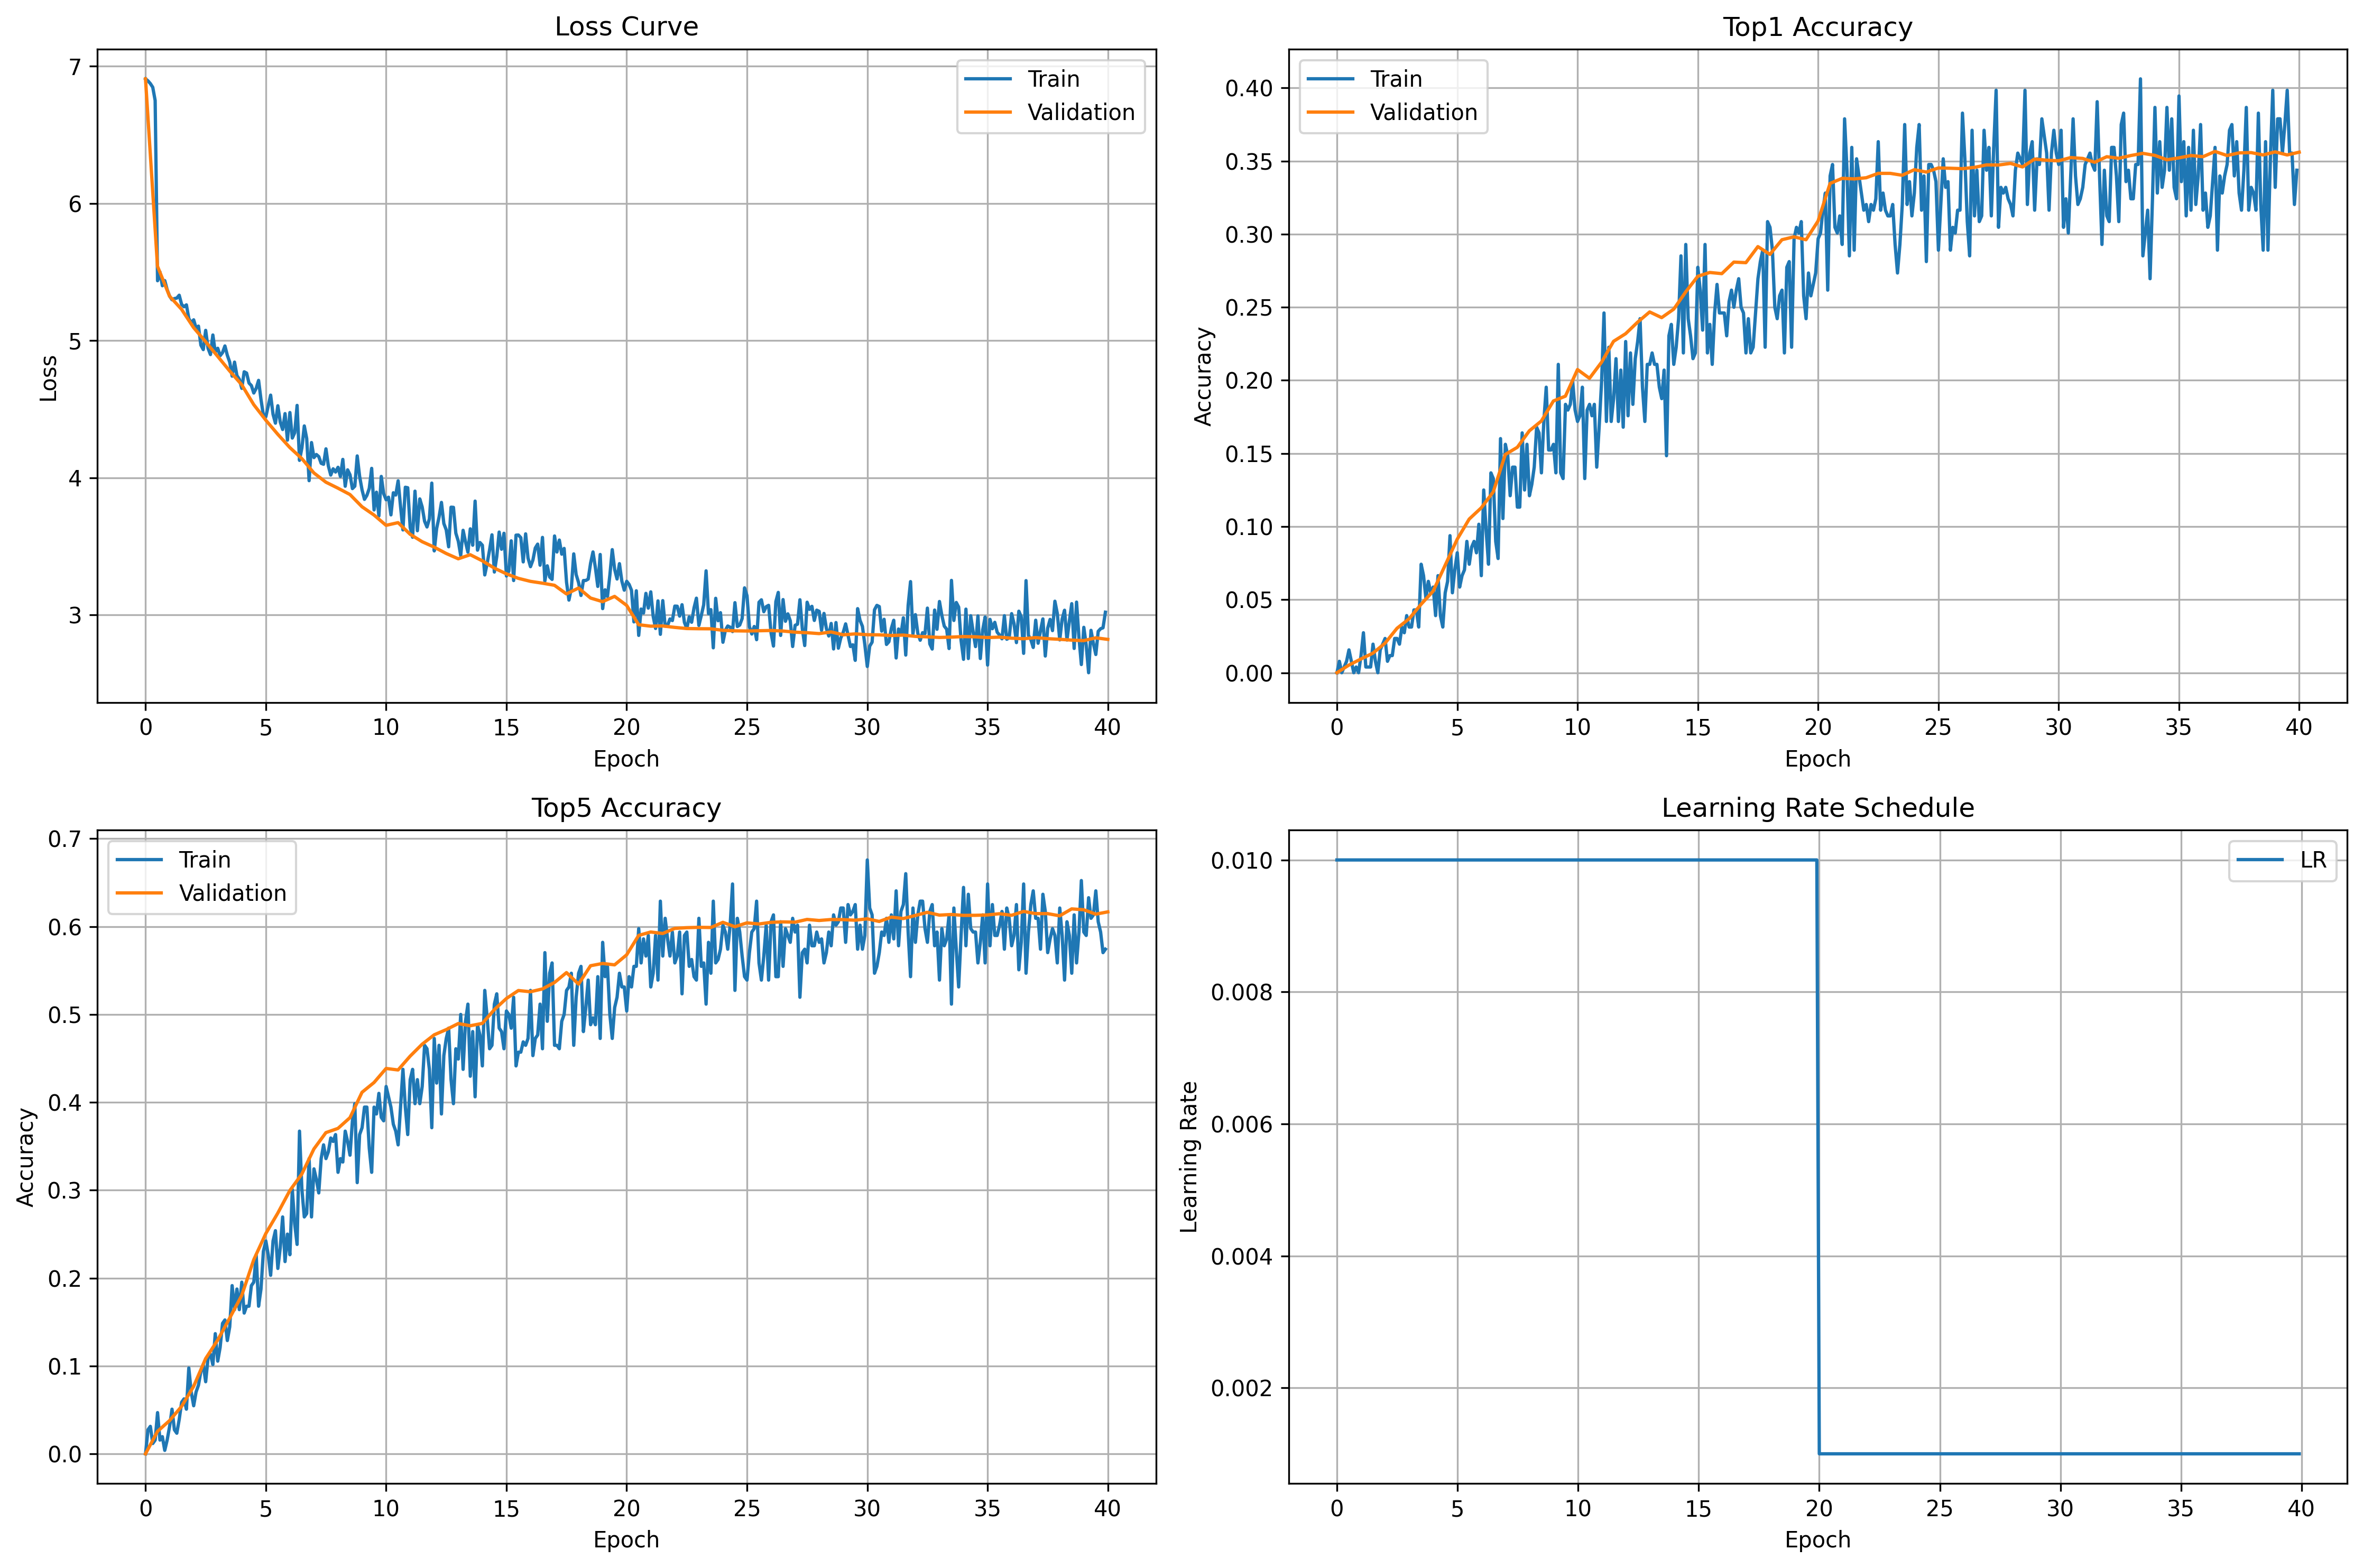
\includegraphics[width=0.9\linewidth]{cornet-z-SE.png}
	\caption{CORnet-Z+SE训练数据变化图}
	\label{f.zsezxt}
\end{figure}

总体来看,SE模块带来的Top-1提升幅度为4.15\%,Top-5提升为3.51\%。虽然提升幅度有限,但考虑到模型结构变化极小,参数量变化可忽略,仍具有实际意义。尤其在训练集上的表现提升表明,注意力机制在训练早期能够加强对有效通道的识别,加快模型收敛速度。

\subsection{小结与分析}

通道注意力机制使模型能够根据全局信息动态调整各通道的响应强度,提升了模型对关键特征的表达能力。训练曲线显示,SE模型在准确率、损失值、学习曲线平稳性等方面均优于原始模型,在保持网络结构轻量的前提下实现了性能上的小幅提升。

不过,相较于大幅度结构重构或多尺度融合模型,本研究采用的改进方式较为保守,性能提升有限。这一结果也说明,通道注意力机制更适合作为辅助增强模块,而非单独主导模型性能的关键因素。
